\documentclass[tikz,border=12pt]{standalone}
\usepackage[american]{circuitikz}
% Shared visual language for standalone EMT block diagrams.
\usepackage{amsmath}
\usetikzlibrary{arrows.meta,backgrounds,calc,fit,positioning}

\tikzset{
    emt diagram/.style = {>={Stealth[length=2.4mm]}},
    line/.style        = {semithick, rounded corners=6pt},
    block/.style       = {draw, semithick, fill=white,
                          minimum height=1cm, minimum width=2.3cm},
    hblock/.style      = {block, minimum width=2.24cm, minimum height=1.3cm},
    vblock/.style      = {block, minimum width=1.3cm, minimum height=2.24cm},
    sum/.style         = {draw, semithick, fill=white, circle,
                          inner sep=2.6pt},
    signal/.style      = {circle, fill, inner sep=1.4pt,
                          label distance=3pt},
    sig/.style         = {font=\small},
    pm/.style          = {font=\scriptsize},
    wire jump/.style   = {line,
                          preaction={draw=white, line width=3pt,
                                     line cap=round}},
    enclosure/.style   = {draw, dashed, semithick, rounded corners=4pt},
    operator enclosure/.style = {enclosure, inner xsep=7mm, inner ysep=6mm}
}


\tikzset{
    igbt/.style = {nigbt, bodydiode, semithick}
}

% TUNABLES: DC rail and switch positions for one representative phase.
\def\railrow{2.25}
\def\switchrow{1.15}

\begin{document}
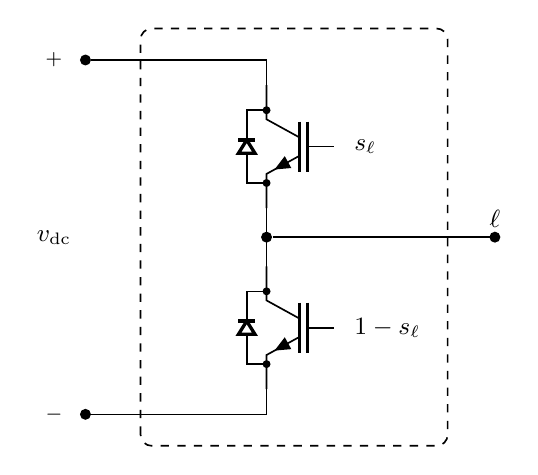
\begin{tikzpicture}[emt diagram]

% ================= DC input =================
\node[signal] (dc+) at (-2.3,\railrow) {};
\node[signal] (dc-) at (-2.3,-\railrow) {};
\draw[line] (dc+) -- (0,\railrow);
\draw[line] (dc-) -- (0,-\railrow);

\node[pm] at (-2.7,\railrow) {$+$};
\node[sig] at (-2.7,0) {$v_{\mathrm{dc}}$};
\node[pm] at (-2.7,-\railrow) {$-$};

% ================= Representative IGBT leg =================
\node[igbt, xscale=-1] (S+) at (0,\switchrow) {};
\node[igbt, xscale=-1] (S-) at (0,-\switchrow) {};
\draw[line] (S+.C) -- (0,\railrow);
\draw[line] (S+.E) -- (0, 0);
\draw[line] (S-.C) -- (0, 0);
\draw[line] (S-.E) -- (0,-\railrow);
\node[sig, anchor=west] at ($(S+.G)+(0.15,0)$) {$s_\ell$};
\node[sig, anchor=west] at ($(S-.G)+(0.15,0)$) {$1-s_\ell$};

% Phase terminal of the representative switching leg.
\node[signal] (phase) at (0,0) {};
\draw[line] (phase) -- (2.9,0) node[signal] {};
\node[sig, above] at (2.9,0) {$\ell$};

% ================= Model enclosure =================
\draw[enclosure] (-1.6,-2.65) rectangle (2.3,2.65);

\end{tikzpicture}
\end{document}
